\chapter{Introduction} \label{cha:Intro}

\section{Regaining Mobility through Wheelchair Assisted Navigation}
The ability to move around to any desired location is critical to all human activity and interaction. With the increase in average age in Western societies, the loss of mobility caused by reduced physical capacity frequently leads to a loss in social contact and therefore quality of life. Given the scale of this phenomenon, reduced mobility should be addressed as a societal problem and not just as one individual's fate \cite{PrasslerEtAl1999}.

The use of robotic technologies can give back a level of mobility and sense of autonomy to the elderly or disabled. An electric-powered wheelchair enables a person with motion impairment to regain movement control and thus re-engage in more frequent human interactions. However, this renewed mobility brings about its own constraints. Wheelchairs are relatively large compared to their indoor environment (corridors, elevators and other narrow passages). In order to realize the fine maneuvers to navigate the chair without colliding in such environment, a significant degree of dexterity is needed. These tasks are even more demanding due to the non-holonomic characteristics of most wheelchairs. It is therefore often a tiresome and frustrating task for elderly and disabled people to control their wheelchair properly \cite{DemeesterEtAl2003}.

Navigation assistance algorithms have been developed to lower the user's workload for maneuvering their wheelchair. This is done by estimating the navigation intention of the driver and modifying driver's actions if needed to obtain a safer path. The secure implementation of assisted navigation requires, however, the correct interpretation of the user's steering signals and the understanding of the static and dynamic environment \cite{DemeesterEtAl2012a}. In order to obtain effective integrated navigation, shared control over the wheelchair movement is required, building on the respective strengths of the driver (for global planning) and the robotic system (for precise motion control) \cite{DemeesterEtAl2003}. 

An electric wheelchair, equipped with sensors needed to perceive the environment and estimate the user's input signals will also be called a semi-Autonomous Mobile Robot (sAMR) or simply robot in this thesis.

\newpage

\section{Current Research at the Department of Mechanical Engineering} \label{sec:CurrentResearch}
\begin{figure}[!htbp]
\centering
\includegraphics[width=0.75\textwidth]{ElectricWheelchair.jpg}
\doublecaption{Example of a commercially available wheelchair upgraded with Navigation Assistance Technology.}{Added are a custom-made haptic interface, laser scanners perceiving the environment and encoders for a more accurate position measurement (from \cite{DemeesterEtAl2012a}). \label{fig:ElectricWheelchair} }
\end{figure} \noindent
The department of Mechanical Engineering of the KU Leuven has already provided significant contributions to the domain of Wheelchair Navigation Assistance through various projects, including the RADHAR project (Robotic ADaptation to Humans Adapting to Robots) \cite{RADHARWebPage}. The following studies \cite{DemeesterEtAl2012b,DemeesterEtAl2012a,DemeesterEtAl2012,VanderPoortenEtAl2012,VanderPoortenEtAl2012a} are briefly presented to introduce the current status of the research and its challenges. The domain of Wheelchair Navigation Assistance can be divided in 3 main research areas: (i) assessment of the navigation intention of the driver; (ii) generation of a local set of feasible paths to model the driver’s navigation intention; and (iii) haptic feedback for shared control, needed for a better interaction between the driver and the motion controller. These are discussed respectively in \cref{sec:PlanRec,sec:ColFreeTraj,sec:SharedControl}. But first, a brief overview of the robotic platform is given in \cref{sec:WheelchairPlatform}.

\subsection{Wheelchair Platform} \label{sec:WheelchairPlatform}
This section discusses the kinematic model of the wheelchair, the constraints to defining feasible trajectories as well as the mapping of the joystick deflection to an executed motion by the wheelchair.
\subsubsection{Wheelchair Kinematic Model}
The electric-powered wheelchair used at the Department of Mechanical Engineering (shown in \cref{fig:ElectricWheelchair}) is a differentially driven vehicle controlled with a joystick. The rotational speed of the two driven wheels can be controlled separately ($u_{right},u_{left}$). The relation between the linear ($v$) and angular ($\omega$) velocity of the wheelchair and the rotational speed of the wheels is given in \cref{eq:DifferentialDriveModel}. ($v,\omega$) are taken with respect to the local wheelchair coordinates frame ($\{R\}$). The equation on the right relates the linear velocity with the angular velocity and the turning radius ($r$), which is also shown in \cref{fig:DifferentialDriveModel} \cite{VanderPoortenEtAl2012}. 

The non-holonomicity of the wheelchair is expressed in \cref{eq:NonHolonDiffDrive}. The wheelchair can only move (instantaneously) in a straight line (along $x_R$) with respect to the local reference frame ($\{R\}$) and/or turn $(\theta_I)$ with respect to an inertial frame ($\{I\}$). This causes challenging situations for the user when performing maneuvers (e.g. passing through a narrow doorway). In addition to the forward-driven wheels, there are also castor wheels, which are not actuated and rotate freely, adapting the driving direction of the wheelchair. These wheels stabilize the wheelchair, but disturb \cref{eq:DifferentialDriveModel}. Their impact is significant when not orientated in the direction of the wheelchair \cite{VanderPoortenEtAl2012}.

To obtain the position with respect to the fixed inertial frame ($\{I\}$), the linear and angular velocities should be integrated as shown in \cref{eq:InertialReferenceFrame}. A visual representation of this is presented in \cref{fig:InertialReferenceFrame}. 

\begin{figure}[!htbp]
\centering
\includegraphics[width=0.5\textwidth]{InertialReferenceFrame.pdf}
\doublecaption{Position and orientation of the sAMR with respect to the inertial reference frame ($\{I\}$).}{\label{fig:InertialReferenceFrame}}
\end{figure}

\begin{align}
v &= \frac{r_{wheel}(u_{right} + u_{left})}{2} & \omega &= \frac{r_{wheel}(u_{right} - u_{left})}{B} & v &= r \cdot \omega \label{eq:DifferentialDriveModel} \\
\dot{x}_R &= v & \dot{y}_R &= 0 & \dot{\theta}_I &= \omega \label{eq:NonHolonDiffDrive} \\
x_I &= \int v(t) \cdot \cos \theta_I(t) \, dt & y_I &= \int v(t) \cdot \sin \theta_I(t) \, dt & \theta_I &= \int \omega(t) \, dt \label{eq:InertialReferenceFrame}
\end{align}

\begin{figure}[!htbp]
\centering
	\begin{minipage}[b]{.45\linewidth}
		\centering
		\includegraphics[width=\textwidth]{DifferentialDriveModel.pdf}
	\end{minipage}
	\hfill%
	\centering
	\begin{minipage}[b]{.5\linewidth}
		\centering
		\includegraphics[width=\textwidth]{JoystickWheelchair.pdf}
	\end{minipage}\\[-7pt]
	\begin{minipage}[t]{.45\linewidth}
		\doublecaption{Differential drive model of the wheelchair.}{At each instant, the turning radius $r$ is determined by the rotational velocities of the wheels. If both are equal and in the same direction, the wheelchair will go straight ($ r= \infty $). If both are equal but in opposite direction, the wheelchair will turn on the spot ($r=0$).  \label{fig:DifferentialDriveModel}}
	\end{minipage}
	\hfill
	\begin{minipage}[t]{.5\linewidth}
		\doublecaption{Joystick deflection used to control the wheelchair.}{Each deflection of the joystick ($x_j,y_j$) with respect to the joystick reference frame $\{j\}$ corresponds to a particular circular motion ($v,\omega$) executed by the wheelchair. The slashed-line on the $\{j\}$ frame corresponds to one particular circular path with radius $r$ drawn in dotted lines. The speed and direction is determined by the position $r_j$ (adapted from \cite{VanderPoortenEtAl2012}). \label{fig:JoystickWheelchair} }
	\end{minipage}\\[-14pt]
\end{figure}

\subsubsection{Kinematic Constraints}
In addition to the non-holonomic constraints, further constraints are implemented to obtain paths comfortable to the user. Although a differential drive robot does not suffer from restrictions on the minimum turning radius as a car-like vehicle, a limit on the minimum turning radius ($r$) is implemented. This, to avoid discomfort to the user due to the large centripetal acceleration caused by a small turning radius ($a_c= r^{-1} \cdot v^2$). Based on the guidelines for human-comfortable navigation \cite{MoralesEtAl2013}, a limit on the minimal turning radius ($r \geqslant 1~m$) is introduced (same as in \cite{DemeesterEtAl2003}). Turning on the spot is allowed only if the wheelchair is not in motion.

\subsubsection{Wheelchair Motion Input}
The user can transmit his commands by using a 2 Degree Of Freedom (DOF) joystick shown in \cref{fig:JoystickWheelchair}. The deflection of the joystick $(x_j,y_j$) with respect to the joystick reference frame ($\{j\}$) will directly correspond to a desired linear and angular velocity of the wheelchair as shown in \cref{eq:InputJoinsic}. ($ k_v,k_{\omega}$) are tuneable velocity gains. Each joystick position corresponds therefore to a circular path with radius $r=|v / \omega|$ taking at a speed proportional to $r_j=\sqrt{x^2_j+y^2_j}$. The slashed line in \cref{fig:JoystickWheelchair} corresponds to the dotted circular path taken at different speeds and directions (forwards or backwards) \cite{VanderPoortenEtAl2012}.

\begin{align}
v &= k_v \cdot y_j & \omega &= -k_{\omega} \cdot x_j \label{eq:InputJoinsic}
\end{align}

\subsection{Plan Recognition} \label{sec:PlanRec}
To improve the assistance provided, the navigation intention of the driver is estimated. The intention at time instant $k$ ($\bm{i_k}$) can be expressed as a succession of desired robot states to a goal state $\bm{i_k} = \{\bm{x_{current}}, \cdots,\bm{x_{goal}}\}$. The robot state is defined as $\bm{x} = [x,y,\theta,v,\omega]^T$. 

To generate a set of plans which will serve as a hypothesis for the user intention, possible goal states are connected with feasible trajectories (the latter will be discussed in the next section). Goal states can be known a priori, by asking a user to indicate them on a map or can be generated by recording places where the user stops regularly.

The last step is to assign and update a certain probability ($p$) for each calculated plan as shown in \cref{eq:PathProbUser}. Bayes' theorem is used to compute the posterior probability on $\bm{i_k}$ which is dependent on the user actions sent ($\bm{u}_k$) and a history ($\bm{\mathcal{H}}$) of the user inputs, robot actions, robot poses and sensor readings. $p_{prior}$ is the previous probability distribution on the set of paths and $p_{user}$ is a user model, based on how the user transforms a particular intention into a certain input. This model is calibrated by asking the user to follow a predefined path. $\eta$ is a scale factor normalizing the probability distribution \cite{DemeesterEtAl2012a}.

\begin{equation}
p_{post}(\bm{i}_k | \bm{u}_k, \bm{\mathcal{H}}_{0:k}) = p_{user}( \bm{u}_k | \bm{i}_k , \bm{\mathcal{H}}_{0:k}) \cdot p_{prior}(\bm{i}_k | \bm{\mathcal{H}}_{0:k}) \cdot \eta \label{eq:PathProbUser}
\end{equation}

\subsection{Collision-Free Trajectories} \label{sec:ColFreeTraj}
In order to assess whether a user input signal is collision-free, it is compared to a precomputed set of discrete motions. These motions consists of a set of circular paths defined by ($v,\omega$) pairs. Each precomputed path is associated with a time ($dt$) before a collision occurs while taking this path, which is continuously updated. A path yielding a low $dt$ is considered dangerous and will therefore be subject to a higher correction by the controller \cite{DemeesterEtAl2012}. The way a controller executes this action will be discussed in the next section. \Cref{fig:NavIntSum} shows the collision-free trajectory generation (left) and plan recognition (right).

\begin{figure}[!htbp]
\centering
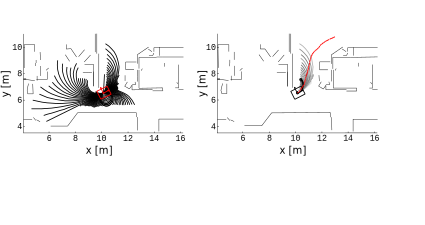
\includegraphics[width=0.8\textwidth]{NavIntSum.pdf}
\doublecaption{Plan recognition based on collision-free trajectories.}{\newline(left) Collision-free trajectories are drawn from the current pose of the robot. (right) Each considered path receives a certain probability (grey-scale, darker color indicates a higher probability). The thick dark precomputed path is locally the best trajectory corresponding to the path (in red) the user will follow (adapted from \cite{DemeesterEtAl2012a}).}
\label{fig:NavIntSum}
\end{figure}

\newpage

\subsection{Shared Control with Haptic Feedback} \label{sec:SharedControl}
When adopting a more traditional scheme of shared control, the user has no direct interaction with the motion controller during the decision-making process. He will only perceive the decided trajectory during the motion of the robot. This can lead to mode confusion \cite{Lankenau2001}, when the path taken by the robot is not the user’s intended plan and even complicates the maneuvering of the wheelchair. This unilateral decision-making scheme is displayed in \cref{fig:SharedControlUni} \cite{VanderPoortenEtAl2012a}. 

To overcome these frustrating situations and to provide a better cooperation between the motion controller and the user, a haptic interface can be used as communication channel. When the current trajectory corresponding to the deflection of the joystick yields a collision in the near future, the haptic interface will provide feedback to the user by ``pushing'' the joystick to a safer direction, while keeping the intention of the user in mind. This interface needs an adapted joystick, featuring additional actuators to provide a certain force ($F_x, F_y$) on the joystick. The user feels at each moment which corrections the controller wants to apply, but is also able to overrule this decision, by applying a higher force as the haptic feedback system, in case a certain direction does not comply with his intention. This bilateral decision-making scheme is displayed in \cref{fig:SharedControlBi} \cite{VanderPoortenEtAl2012a}. 

\begin{figure}[!htbp]
\centering
	\begin{minipage}[b]{.45\linewidth}
		\centering
		\includegraphics[width=\textwidth]{SharedControlUni.pdf}
	\end{minipage}
	\hfill%
	\centering
	\begin{minipage}[b]{.45\linewidth}
		\centering
		\includegraphics[width=\textwidth]{SharedControlBi.pdf}
	\end{minipage}\\[-7pt]
	\begin{minipage}[t]{.45\linewidth}
		\doublecaption{Unilateral decision-making schemes}{don't involve the user in the final decision which can lead to confusion if the selected motion doesn't correspond to the user’s desired motion. Moreover, the user only notices what he perceives as an error in interpretation after the wheelchair has moved (from \cite{VanderPoortenEtAl2012a}). \label{fig:SharedControlUni}}
	\end{minipage}
	\hfill
	\begin{minipage}[t]{.45\linewidth}
		\doublecaption{Bilateral decision-making schemes}{using haptic feedback inform the user of the chosen navigation direction by forcing the joystick to the corresponding position of that motion. If the motion doesn't comply with the user's intention, he can overrule it by forcing the joystick towards his desired position (from \cite{VanderPoortenEtAl2012a}). \label{fig:SharedControlBi}}
	\end{minipage}
\end{figure}

\newpage
\section{Scope and Contribution} \label{sec:contribution}
There is a certain lack of flexibility when only employing circular curves to calculate collision-free trajectories, since circular paths are only a small subset of all feasible motions. When the wheelchair has to pass through a narrow space, from an unfavorable pose as depicted in \cref{fig:EntranceRobotLab} (left) the Local Path Planning Algorithm (LPPA) based on circular arcs only does not find a path going through the doorway. This limits the assistance provided to the user.

This thesis will expand the set of feasible motions by using a more complex curve geometry, thereby offering higher flexibility by being less dependent on the actual pose of the robot as illustrated in \cref{fig:EntranceRobotLab} (right). However, such increased flexibility should be provided while still ensuring fast and accurate collision checking as this has to be performed online. It is therefore important to find a systematic way to create this new set of paths, such that intuitive design parameters can be tuned depending on the complexity of the environment through which the sAMR has to navigate.

\begin{figure}[!htbp]
\centering
	\begin{minipage}[b]{.45\linewidth}
		\centering
		\includegraphics[width=\textwidth]{EnterRobotLabCirc.pdf}
	\end{minipage}
	\hfill%
	\centering
	\begin{minipage}[b]{.45\linewidth}
		\centering
		\includegraphics[width=\textwidth]{EnterRobotLabCloth.pdf}
	\end{minipage}
	\doublecaption{Finding collision-free paths through a narrow doorway depends on the used curve geometry.}{(left) Limited guidance is offered to the user when the collision-free trajectories are only based on circles, as they only represent a limited subset of the feasible paths. (right) Employing curves offering more flexibility will result in feasible paths going through the narrow doorway, thus providing better navigation assistance to the user, less dependent on the current pose of the sAMR. \label{fig:EntranceRobotLab}}
\end{figure}

Two other aspects will also be presented to further improve the LPPA: (i) a conceptual solution to compute the velocity profile for each local path in a dynamic environment given a motion model of the moving objects; (ii) considerations to obtain a socially compliant path planner are developed and the methods needed to enable a planning algorithm in dense crowded environments are shown.

The next section aims to provide an overview of the different aspects that can be considered when designing a Local Path Planner (LPP) and will outline the aspects that will be addressed in this thesis.

\newpage

\section{Requirements for a Local Path Planner} \label{sec:ReqLPP}
%TODO
% Find castor wheels and uncertenties
The task of the LPP is to identify the paths that will be selected in the immediate future. In the context of Wheelchair Navigation Assistance, the LPP also plays the role of providing several feasible trajectories used to model the user's intention. Several additional aspects can be considered to design a reliable LPP in this context. Based on recent literature, these can include: 
\vspace{1em}
\begin{enumerate}
\item Improving user’s intention estimation by widening the range of possible paths \cite{DemeesterEtAl2012,VanderPoortenEtAl2012}.
\item Increase the capacity of the LPP to calculate efficiently more complex paths to assist a wider range of maneuvers in crowded environments including parallel parking and three-point turns for a 180° change in direction \cite{DemeesterEtAl2012,PivtoraikoEtAl2009,ZipsEtAl2016}.
\item Taking into account robot geometry, kinematics and dynamics for path calculations close to the current position of the robot \cite{BouraineEtAl2011,DemeesterEtAl2012,PivtoraikoEtAl2009}.
\item Human-aware path planning, which would greatly improve the effectiveness of navigation in dynamic and crowded environments \cite{KruseEtAl2013,TrautmanEtAl2015}.
\item Accounting for the impact of castor wheels on possible trajectories.
\item Improvements in the way to deal with uncertainties (e.g. in path execution, due to discretisation, etc.) \cite{BouraineEtAl2011,MercyEtAl2016}.
\end{enumerate}
\vspace{1em}

From the above list, this thesis will focus on point 1 and therefore implicitly assist with point 2, when using Discrete Motion Planning (DMP). Point 3 will be partially addressed by providing a conceptual solution for dynamic obstacle avoidance. The paths and collision avoidance will take into account the robot geometry and kinematics. Possible solutions to address point 4 will be presented, to obtain a socially compliant path planner.

\section{Overview} \label{sec:overview}
This thesis is structured as follows: a literature study on path planning algorithms and human-aware navigation is presented in \cref{cha:LitStudy}, providing a review of several methods to generate a set of flexible trajectories and of guidelines to obtain a more socially compliant navigation. The design of a novel LPPA is detailed in \cref{cha:Design} followed by an evaluation of that design in \cref{cha:Eval}. Future work as well as a conclusion of this thesis can respectively be found in \cref{cha:FutWork,cha:Concl}.

There are also two appendices, \cref{app:BezierCurve} further elaborates mathematical concepts of the Bézier curve, one of the considered curves for motion planning. Finally, the content of the source code of the GitLab repository \cite{Denis2017} containing the same information as the digital appendix, is presented in \cref{app:SourceCode}